\newpage
\section{Calibration}
\subsection{Required}
For the calibration procedure it's required some kind of resistive load that will load the port's power out. This can be done from a device as it's show at figure~\ref{fig:calibrator_top}.
\begin{figure}[h!]
	\centering
	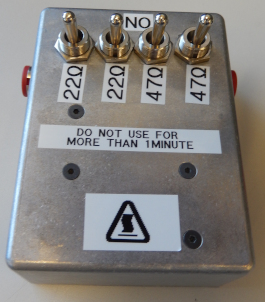
\includegraphics[width=2.5in]{./pics/calibrator_top.jpg}
	\caption{Top view of the Calibrator device}
	\label{fig:calibrator_top}
\end{figure}
The calibration device it's have inside some resistors and some sampling points for the measurements of voltage and current. At figure~\ref{fig:calibrator_block} is shown a cartoon type diagram
of the calibrator device.
\begin{figure}[h!]
	\centering
	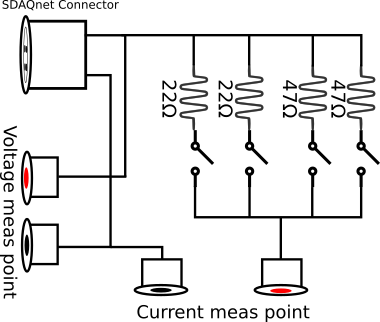
\includegraphics[width=3in]{./Artwork/calibrator_block.png}
	\caption{Calibrator's BLock Diagram}
	\label{fig:calibrator_block}
\end{figure}

For the calibration procedure are required:
\begin{itemize}
	\item The calibration device.
	\item One DMM configured as voltmeter.
	\item One DMM configured as Ammeter.
	\item Banana terminal cables.
	\item A short($\leq10''$) 4pin Lemo cable
\end{itemize}
\newpage
\subsection{Calibration Procedure}
The calibration procedure start by booting the computer that runs the Morfeas system and after finishing of boot continue with a request of stop of the Morfeas system from the systemd.
Then continue by executing the ``Morfeas\_RPi\_Hat" software. Then connect the two DMMs on the calibrator device and the calibrator device to the first port of the computer that is equip with the Morfeas RPi Hat.
All the switches of the calibrator must be open.\\
The first command where is issued is ``set p\# czero" (with all the switches open). This will zero the offset error of the particular CSA. Then the value of voltage out of the channel that displayed
at the DMM is recorded. After of this issue ``set p\# vgain Rec\_Value". This will correct the reading of voltage. After of this calibration of current follow by apply some load to the port.
$3/4$ of the maximum value($4A$) is a good start. The value from the DMM that measure current is recorded and issued as correction with command ``set p\# cgain Rec\_value".
Load now can be removed. A Check for linearity can be done by comparing the readings of DMM and CSA in different load values. A $1\%$ error is the maximum allowed.
In case that this is not satisfied repeat the current calibration with a different load. Otherwise save the configuration with command ``save p\#" and continue by repeating the above for the next port.
After of the calibration finish place a bullet on the ``CAL OK" mark on the front of the PCB
***The ``\#" on the above must be replaced with the number of the Port.\\

All of the above briefly:
\begin{enumerate}
	\item Boot the computer.
	\item Issue stop of the Morfeas System.
	\item Connect DMMs on Calibrator.
	\item Open all switch of the calibrator.
	\item Connect Calibrator with the a port.\label{loop}
	\item Issue ``set p\# czero".
	\item Record the Voltage measurement from DMM.\label{voltage}
	\item Issue ``set p\# vgain Rec\_Value" with the previously recorded value.
	\item Compare measurement DMM with SCA. if error ($>5\%$) go to \ref{voltage} and repeat.
	\item Load the port.\label{current}
	\item Record Value of current from DMM.
	\item Issue ``set p\# cgain Rec\_value" with the previously recorded value.
	\item Check Linearity ($\leq1\%$) by comparing readings of DMM and CSA.\\ if not satisfied go to \ref{current} and repeat.
	\item Issue ``save p\#" to save the port's configuration to EEPROM.
	\item Go to \ref{loop} and repeat for next port.
	\item Mark ``CAL OK". 
	\item Issue Start of the Morfeas System.
	\item Done.
\end{enumerate}
